\documentclass[]{beamer}
% Class options include: notes, notesonly, handout, trans,
%                        hidesubsections, shadesubsections,
%                        inrow, blue, red, grey, brown

% Theme for beamer presentation.
\usepackage{beamerthemesplit} 
\usepackage{tabularx}
\usepackage{epstopdf}
\usepackage{amsmath}
\usepackage{subfig}
\makeatletter

\def\hlinewd#1{%
\noalign{\ifnum0=`}\fi\hrule \@height #1 %
\futurelet\reserved@a\@xhline}
\makeatother

\newenvironment{changemargin}[2]{%
  \begin{list}{}{%
    \setlength{\topsep}{0pt}%
    \setlength{\leftmargin}{#1}%
    \setlength{\rightmargin}{#2}%
    \setlength{\listparindent}{\parindent}%
    \setlength{\itemindent}{\parindent}%
    \setlength{\parsep}{\parskip}%
  }%
  \item[]}{\end{list}} 
% Other themes include: beamerthemebars, beamerthemelined, 
%                       beamerthemetree, beamerthemetreebars  
\newcommand{\tab}{\hspace*{2em}}
\newcommand*\oldmacro{}%
\let\oldmacro\insertshorttitle%
\renewcommand*\insertshorttitle{%
  \oldmacro\hfill%
  \insertframenumber\,/\,\inserttotalframenumber}
\title{Malware Reverse Engineering}    % Enter your title between curly braces
\author{Andrea Mambretti (m4mbr3@gmail.com)}        % Enter your name between curly braces
\institute{Politecnico di Milano}      % Enter your institute name between curly braces
\date{\today}                    % Enter the date or \today between curly braces

\begin{document}

% Creates title page of slide show using above information
\begin{frame}
  \titlepage
\end{frame}
\note{Talk for 50 minutes} % Add notes to yourself that will be displayed when
                           % typeset with the notes or notesonly class options

\section[Outline]{}

% Creates table of contents slide incorporating
% all \section and \subsection commands
\begin{frame}
  \tableofcontents
\end{frame}
\section {Crash course on Assembly Language}
	\subsection{Overview on the common 32-bit Intel Architecture (IA)}
		\begin{frame}
			\frametitle{(1) How is the IA made?}
			\begin{itemize}
				\item{The processor has 32 bits internal registers to manage and execute operations on data\newline They are EAX, EBX, ECX, EDX, ESI, EDI, EBP, EIP and ESP }
				\item{Among them we identify EAX, EBX, ECX, EDX are for general purpose}
				\item{EBP (BP = base pointer) and ESP (SP = stack pointer) are the stack bounds }
				\item{EDI and ESI are extra-registers}
				\item{EIP (IP = instruction pointer) is the register that contains the address of the next instruction}
			\end{itemize}
		\end{frame}
		\begin{frame}
			\frametitle{(2) How is the IA made?}
			\begin{columns}
				\begin{column}[left]{2.5in}
					\begin{figure}
						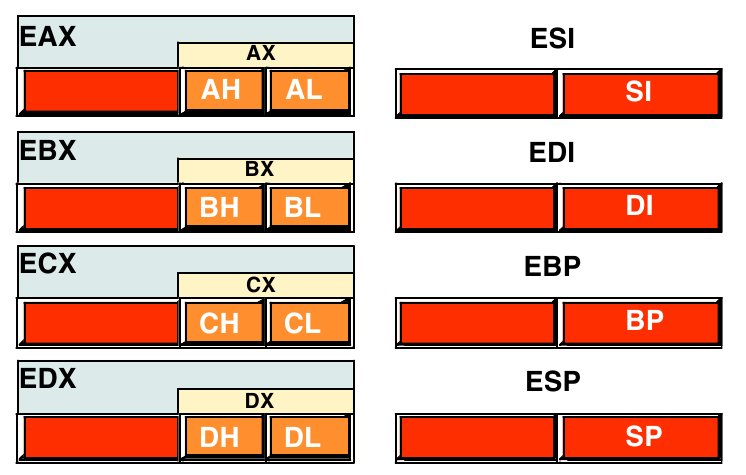
\includegraphics[height=1.6in]{images/registers.jpeg}
						\label{Registers Division}
					\end{figure}
				\end{column}
				\begin{column}[right]{2.5in}
					\begin{itemize}
							\item{The register name system is a porting from 16-bit IA where the registers were called AX, BX and so on.\newline "E" means extended. Without it we consider the corrisponding 16-bit register\newline There's also the possibility to use AX,BX,CX,DX such as 8-bit registers. For example we can use AX as AH and AL that mean higher and lower 8 bits of AX}
					\end{itemize}
				\end{column}
			\end{columns}
		\end{frame}
		\begin{frame}
			\frametitle{(1) What about EFLAGS?}
			\begin{figure}
				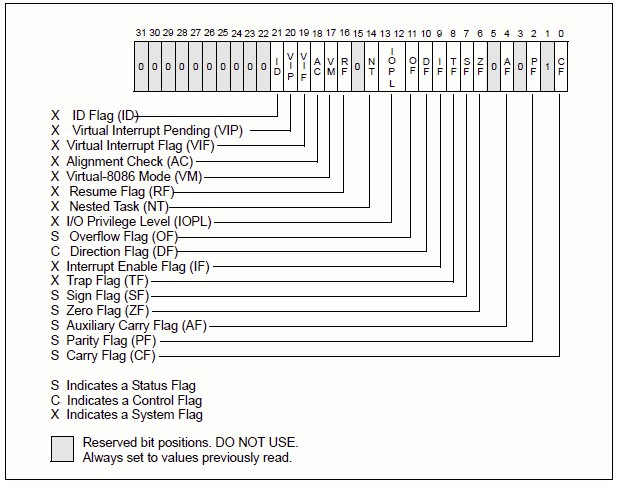
\includegraphics[height=2.5in]{images/eflags.jpeg}
				\label{Eflags idea}
			\end{figure}
		\end{frame}
		\begin{frame}
			\frametitle{(2) What about EFLAGS?}
			\begin{itemize}
				\item{It's another 32-bit register}
				\item{Only 8 bits out of 32 are of interest for us. The others are either for the kernel mode function or  are of little interest for programmers}
				\item{The 8 bits are called flags. We consider them singularly. They are boolean (true/false) }
				\item{The meaning of each bit is different. They represent overflow, direction, interrupt disable, sign, zero, auxiliary carry, parity and carry flags}
				\item{Since they represent information about the instruction last executed, they change at every execution step. They are VERY important for the control flow of the program }				
			\end{itemize}
		\end{frame}
	\subsection{Overview on different syntaxes}
		\begin{frame}
			\frametitle{Syntax}
			\begin{itemize}
				\item{In the assembly world we can find two main syntaxes: the AT\&T and the Intel}
				\item{AT\&T syntax is used by all UNIX program (e.g. gdb)}
				\item{Intel syntax is used by Microsoft programs (IDApro and others)}
			\end{itemize}
		\end{frame}
		\begin{frame}
			\frametitle{(1) Differences in the notation}
			\begin{itemize}
				\item{Consider the following operation:\newline\centerline{"move the value 0 to EAX"}}
				\item{AT\&T: \centerline{ mov \$0x0,\%eax} }
				\item{Intel: \centerline{ mov eax, 0h}}
				\item{Comments:} 
				\begin{itemize}
					\item{As you can see in AT\&T syntax the destination is the second operand instead as in the Intel syntax}
					\item{In the AT\&T syntax the register are denoted with \% and the immediate/costant with \$. In the Intel syntax these tokens are not used. }
				\end{itemize}
			\end{itemize}
		\end{frame}
		\begin{frame}
			\frametitle{(2) Differences in the notation}
			\begin{itemize}
				\item{Consider this new operation:\newline\centerline {"move the value 0 to the address contained in EBX+4"}}
				\item{AT\&T: \centerline{ mov \$0x0,0x4(\%ebx)}}
				\item{Intel: \centerline{ mov [ebx+4h],0h }}
				\item{Comments:}
				\begin{itemize}
					\item{This case shows how  the deferentiation is done in assembly}
					\item{In AT\&T we use parenthesis. In the Intel syntax we have to use square brackets}
					\item{The way to manage the offset is another syntax difference. In the first case we have to put it out of the parenthesis in the second one inside the square brackets }
				\end{itemize}
			\end{itemize}
		\end{frame}
	\subsection{Basic Instructions}
		\begin{frame}
			\frametitle{(1) Basic instructions overview}
				\begin{itemize}
					\item{Every processor has a huge instruction set (see Intel Manual\footnote{\url{http://www.intel.com/content/www/us/en/processors/architectures-software-developer-manuals.html}})}
					\item{A subset of the whole instruction set is usually processor dipendent}
					\item{We will focus on the other subset of instructions that is common among the processors}
					\item{We will use the Intel syntax as it is the same syntax used in IDApro by default}
				\end{itemize}
		\end{frame}
		\begin{frame}
			\frametitle{(2) Basic Instruction MOV}
				\begin{itemize}	
					\item{ General: MOV \underline{\textbf{destination}}, \underline{\textbf{source}}}\\
					\textbf{source} can be an immediate, a register, a memory location\\
					\textbf{destination} can be either a register  or a memory location\\
					NB: Every combination is possible except memloc to memloc!!!It isn't valid here and in all the instructions!!!

					\item{With this instruction, as said in the example above, we move a value from a source place to a destination. There are a ton of different versions. They change in function of the operands ex 32 bits operands, 16 bits operands, immediate to reg, immediate to memory }
				\item{Examples}
					\begin{table}[h]
						\begin{tabular}{|c|c|c|}
							\hline
							MOV eax, ebx&MOV eax, FFFFFFFFh &MOV ax, bx\\    \hline
							MOV [eax],ecx&MOV [eax],[ecx] \color{red}NO!!!&MOV al, FFh\\
							\hline
						\end{tabular}
					\end{table}
			\end{itemize}	

		\end{frame}
		\begin{frame}
			\frametitle{(3) Basic Instruction ADD}
			\begin{itemize}
					\item{General: ADD \underline{\textbf{destination}}, \underline{\textbf{source}}}\\
					\textbf{source} can be an immediate, a register, a memory location\\
					\textbf{destination} can be either a register or a memory location\\
					NB: The destination register has to be as big as at least the source or greater 
					\item{With this instruction we can add a value from \textbf{source}  to the destination operand and put the new value inside the destination}
					\item{Examples}
					\begin{table}[h]
						\begin{tabular}{|c|c|c|}
							\hline
							ADD esp, 44h&ADD eax, ebx&ADD al, dh\\
							\hline
							ADD  edx, cx&ADD [eax],[ecx] \color{red}NO!!!&ADD [eax],1h\\
							\hline
						\end{tabular}
					\end{table}

			\end{itemize}
		\end{frame}
		\begin{frame}
			\frametitle{(4) Basic Instruction SUB}
			\begin{itemize}
				\item{General: SUB \underline{\textbf{destination}}, \underline{\textbf{source}}}\\
				\textbf{source} can be an immediate, a register, a memory location\\
				\textbf{destination} can be either a register or a memory location\\
					NB: The destination register has to be as big as at least the source or greater 
				\item{With this instruction we can subtract the value \textbf{source}  from the destination operand and put the new value inside the destination}

				\item{Examples}
					\begin{table}[h]
						\begin{tabular}{|c|c|c|}
							\hline
							SUB esp, 33h&SUB eax, ebx&SUB al, dh\\
							\hline
							SUB edx, cx&SUB [eax],[ecx] \color{red}NO!!!&SUB [eax],1h\\
							\hline
						\end{tabular}
					\end{table}

			\end{itemize}
		\end{frame}
		\begin{frame}
			\frametitle{(5) Basic Instruction MUL}
			\begin{itemize}
				\item{General: MUL \underline{\textbf{Operand}}}\\
				\textbf{Operand} can be an immediate, a register, a memory location\\

				\item{With this instruction we can multiplies \textbf{Operand} by the value of corresponding byte-length in the EAX,AX,AL register }
					\begin{table}[h]
						\begin{tabular}{|c!{\vrule width 1pt}c|c|c| }
							\hline
							OperandSize:& 1 byte & 2 bytes& 4 bytes\\	\hlinewd{1.3pt}
								Other Operand& AL     & AX   & EAX\\	\hline
							Higher Part of result: & AH & DX & EDX\\		\hline
							Lower Part of result:  & AL & AX & EAX\\
							\hline
						\end{tabular}
					\end{table}

					\item{Examples}
					\begin{table}[h]	
						\begin{tabular}{|c!{\vrule width 1pt}c|c|c|}
							\hline
							OperandSize:&1 byte & 2 bytes & 4 bytes\\ \hlinewd{1.3pt}

							Immediate&MUL 44h & MUL 4455h & MUL 44556677h\\ \hline
							Register&MUL cl & MUL dx & MUL ebx \\
							\hline
						\end{tabular}
					\end{table}
			\end{itemize}
		\end{frame}

		\begin{frame}
			\frametitle{(6) Basic Instruction DIV}
			\begin{itemize}	
				\item{General: DIV \underline{\textbf{Operand}}}\\
				\textbf{Operand} can be an immediate, a register, a memory location

				\item{With this instruction we can divide the value in the dividend register(s) by "Operand"}
					\begin{table}[h]
						\begin{tabular}{|c!{\vrule width 1pt}c|c|c| }
							\hline
							OperandSize: & 1 byte & 2 bytes & 4 bytes\\	\hlinewd{1.3pt}
							Dividend     & AX     & DX:AX   & EDX:EAX\\	\hline
							Remainder  & AH & DX & EDX\\		\hline
							Quotient  & AL & AX & EAX\\							\hline
						\end{tabular}
					\end{table}
					\item{Examples}
					\begin{table}[h]	
						\begin{tabular}{|c!{\vrule width 1pt}c|c|c|}
							\hline
							OperandSize:&1 byte & 2 bytes & 4 bytes\\ \hlinewd{1.3pt}
							Register&DIV bl & DIV bx & DIV ebx\\ \hline
							Immediate&DIV 66h & DIV 6677h & DIV 66778899h \\
							\hline
						\end{tabular}
					\end{table}
			\end{itemize}
		\end{frame}

		\begin{frame}
			\frametitle{(7) Basic Instruction CMP}
			\begin{itemize}
				\item{General: CMP \underline{\textbf{Operand\_1}}, \underline{\textbf{Operand\_2}}}\\

				\item{This instruction performs a subtraction between two operands and sets  the flags, it doesn't store the result}
				\item{Examples}
					\begin{table}[h]
						\begin{tabular}{|c|c|c|}
							\hline
							CMP eax, ebx&CMP eax, 44BBCCDDh&CMP al, dh\\
							\hline
							CMP al, 44h&CMP ax,FFFFh&CMP [eax],4h\\
							\hline
						\end{tabular}
					\end{table}
			\end{itemize}
		\end{frame}
		\begin{frame}
			\frametitle{(8) Basic Instruction JMP}
				\begin{columns}
					\begin{column}[left]{2.5in}
						\begin{figure}
							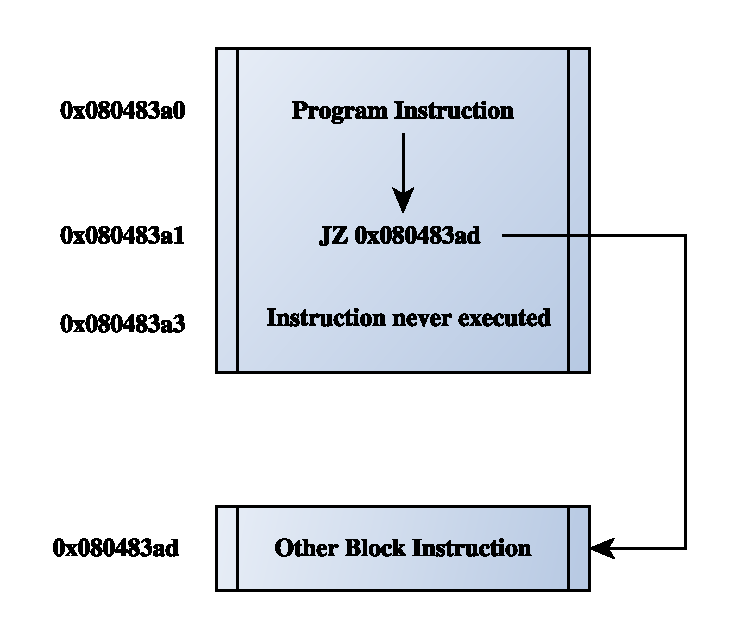
\includegraphics[width=\textwidth]{images/jmp.eps}
							
							\label{Control Flow JMP}
						\end{figure}
					\end{column}
					\begin{column}[right]{2.5in}
						\begin{itemize}	
							\item{General: JMP \underline{\textbf{address}}}\\

							\item{This instruction is called unconditional jump and when is executed put in the eip (the next instruction address) the \textbf{address} passed as operand. We say that the execution jumps to \textbf{address} and it's unconditional because always the execution jump.}
						\end{itemize}

					\end{column}
				\end{columns}
		\end{frame}
		\begin{frame}
			\frametitle{(9) Basic Instruction JZ,JNZ and so on}
				\begin{columns}
					\begin{column}[left]{2.5in}
						\begin{figure}
							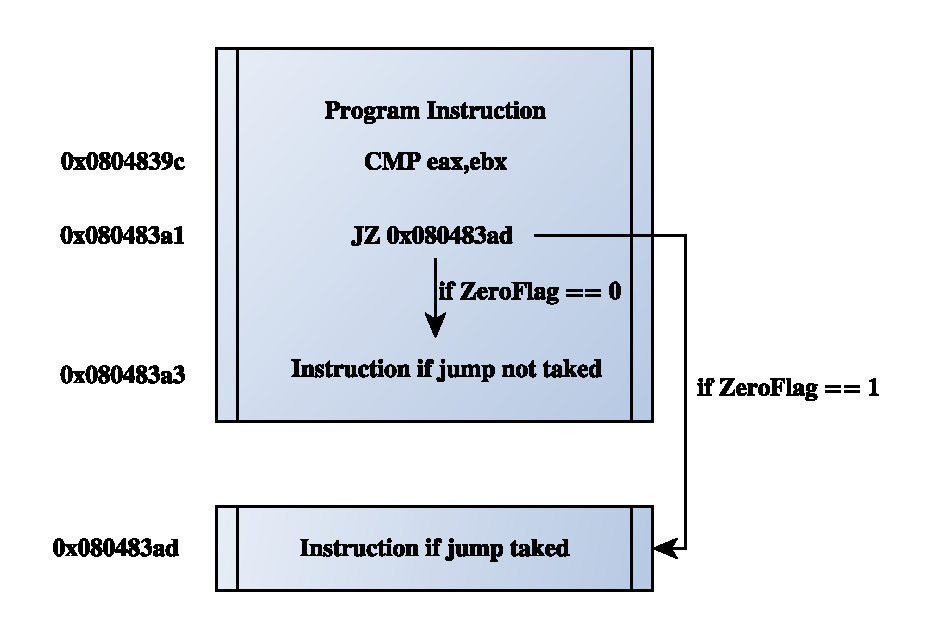
\includegraphics[width=\textwidth]{images/j_unc.eps}									      \label{control}
							\label{Control Flow JZ}
						\end{figure}
					\end{column}
					\begin{column}[right]{2.5in}
						\begin{itemize}
							\item{General: JX \underline{\textbf{address}}}\\
							$ X \in \{O,NO,S,NS,E,Z,NE...\}$\\
							\item{This set of instruction are called conditional jump. It means that the execution will go to \textbf{address} if and only if the specific flag of the condition jump given is verified.\\For example: jz jumps if zero flag is 1 if no is not taked}						\end{itemize}
					\end{column}\footnote{\url{http://www.unixwiz.net/techtips/x86-jumps.html}}

				\end{columns}
		\end{frame}
		\begin{frame}
			\frametitle{(10) Basic Instruction INT}
				\begin{itemize}
					\item{General: INT \underline{\textbf{VALUE}}}\\
					\item{\textbf{VALUE} is the software interrupt that should be generated (0-255)}
					\item{Famous values are 21h for call service under windows and 80 for linux}
					\item{look the manual for the other } 
				\end{itemize}
		\end{frame}
			
	\subsection{x86\_64}
		\begin{frame}
			\frametitle{How much is different x86\_64 from x86?}
			\begin{changemargin}{-0.7cm}{0cm}
			\begin{itemize}
				\item{The prefix of  the register is r instead of e so we have (rip, rax etc.)}
				\item{There are 8 new registers (r8 to r15)}
				\item{each of them can be consider at 8, 16, 32, 64 bits\\
				   with $X \in \{8..15\}$ we have }
				\begin{table}[h]
					\begin{tabular}{|c!{\vrule width 1pt }c|c|c|c|}
					\hline
					bits&8&16&32&64\\
					\hline
					reg&rXb&rXw&rXd&rX\\
					\hline	
					\end{tabular}
				\end{table}
				\item{for better syntax information look at \url{http://www.x86-64.org/documentation/assembly.html}}
			\end{itemize}
			\end{changemargin}
		\end{frame}
\section{Something more}
	\subsection{Program layout in memory}
		\begin{frame}
			\frametitle{Different Binary File Format}
				\begin{itemize}
					\item{\color{red}PE (Portable Executable)\color{black}: This kind of binary file format is used by Microsoft binary executable.}
					\item{\color{red}ELF\color{black}: This is the common binary format for Unix, Linux, FreeBSD and others}
					\item{\color{red}Other\color{black}}
				\end{itemize}
		\end{frame}
	
		\begin{frame}
			\begin{changemargin}{-1cm}{-1cm}
				\frametitle{How a program is seen in memory in linux (\color{red} ELF\color{white})}
					\begin{table}[l]
						\resizebox{12.5cm}{3cm}{

						\scalebox{0.9}{

					\begin{tabular}{|l l|}
						\hlinewd{1pt}
							\textbf{Executable}&\textbf{Description}\\\hlinewd{1.3pt}
							.bss&This section holds uninitialized data that contribute to the program's memory image.\\
							&By definition, the system initializes the data with zeros when the program begins to run.\\\hline
							.comment&This section holds version control information.\\\hline
							.data/.data1& These sections hold initialized data that contribute to \\
							&the program's memory image\\\hline
							.debug&This section holds information symbolic debugging.\\\hline
							.text&This section holds the "text," or executable instructions, of a program.\\\hline
							.init&This section holds executable instructions that contribute to the process initialization code.\\\hline
							&That is, when a program starts to run, the system arranges to execute the code in this\\
							&section before calling the main program entry point (called main for C programs).\\
							\hline
							.got&This section holds the global offset table.\\
							\hline
				
					\end{tabular}
					}
					}
					\end{table}
			\end{changemargin}
		\end{frame}
		
		\begin{frame}
			\begin{changemargin}{-1cm}{-1cm}
				\frametitle{How a program is seen in memory in windows (\color{red} PE\color{white})}
					\begin{table}[l]
						\resizebox{12cm}{3cm}{

						\scalebox{0.9}{
						\begin{tabular}{|l l|}
							\hlinewd{1pt}
								\textbf{Executable}&\textbf{Description}\\\hlinewd{1.3pt}
								.text&Contains the executable code\\\hline
								.rdata&Holds read-only data that is globally accessible within	\\
								&the program\\\hline
				
								.data&Stores global data accessed throughout the program\\\hline
								.idata&Sometimes present and stores the import function information;\\
								& if this section is not present, the import function information\\
								&is stored in the .rdata section\\\hline
								.edata&Sometimes present and stores the export function information;\\								      &if this section is not present, the export function information\\
								& is stored in the .rdata section\\\hline
								.pdata&Present only in 64-bit executables and stores\\
								& execption-handling information\\\hline
								.rsrc&Stores resources needed by the executable\\\hline
								.reloc&Contains information for relocation of library files\\\hline
						\end{tabular}
						}
						}
					\end{table}
			\end{changemargin}
		\end{frame}
		\begin{frame}
			\frametitle{A General Schema}
				\begin{figure}
					\scalebox{0.35}{
					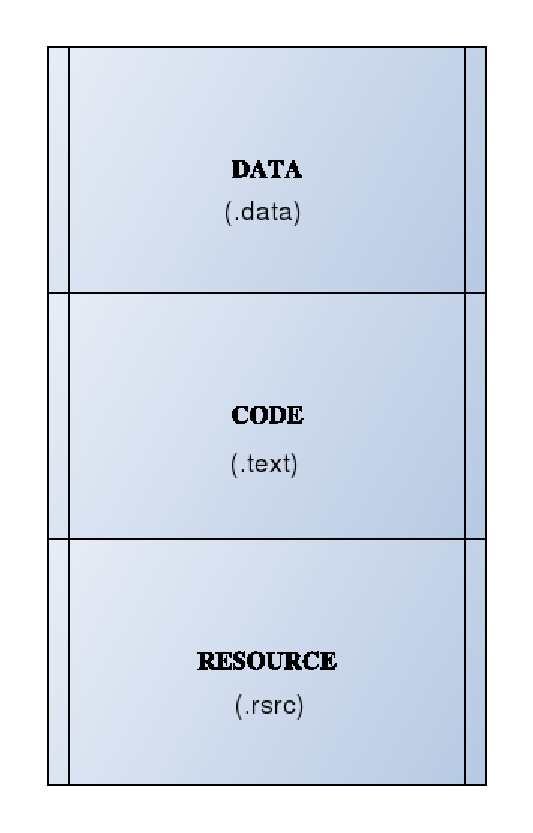
\includegraphics[width=\textwidth]{images/prog_memory.eps}
					\label{The important idea that we must have in mind before looking inside a binary file}
					}
				\end{figure}
		\end{frame}				

\subsection{Function and call convention}
		\begin{frame}
			\frametitle{Function}
			\begin{itemize}
				\item{The concept of function in assembly is the same of the common function in almost all the programming languages }
				\item{Is a piece of code that receive data from the caller a return some value after the elaboration}
				\item{Differently from all high level languages the way to pass parameters to a function can be done in more than one way}
				\item{Is different also the way how to call a specific function}
			\end{itemize}
		\end{frame}
		\begin{frame}
			\frametitle{Function, An example}
				\begin{figure}
					\scalebox{0.54}{
					\includegraphics[width=\textwidth]{images/function.eps}
					\label{A Function Example}
					}
				\end{figure}
		\end{frame}
		\begin{frame}
			\frametitle{Call Convention}
			\begin{itemize}
				\item{It's the way how a program receives parameters,how a function returns its return value and who cleans the stack}
				\item{There are different implementation of the Call Convention that dictates exactly where a caller should place any parameters that a function requires}
				\item{Everything is dipendent by the compiler(gcc/g++, visual studio c++ etc.) and by the high-level language from which the assembly comes from (c, c++, visualbasic and so on) }
				\item{Let's look at some of those}
			\end{itemize}
		\end{frame}
		\begin{frame}
			\frametitle{The C Calling Convention}
			\begin{itemize}
				\item{It's the default calling convention used by most C compilers for the x86 arch}
				\item{When a compiler doesn't use this convention we can force it using the modifier \color{red}\_cdecl}
				\item{It specifies that the \textbf{caller place} parameters to a function on a stack in the right to left order and that the \textbf{caller remove} the parameters from the stack after the called function completes}
			\end{itemize}
		\end{frame}
		\begin{frame}
			\frametitle{The C Calling Convention example}
			\begin{figure}
				\subfloat{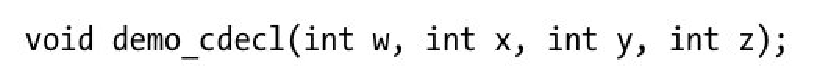
\includegraphics[width=7cm]{images/demo_cdecl.eps}}\\
				\begin{columns}
					\begin{column}[center]{2.5in}
						\subfloat{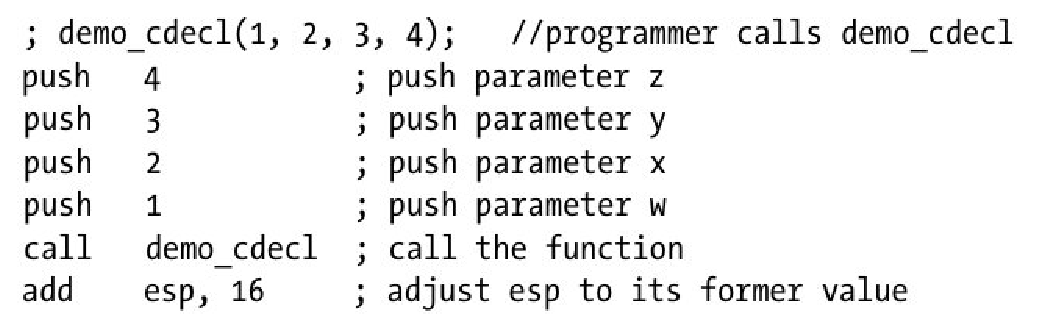
\includegraphics[width=7cm]{images/cdecl_place.eps}}\\
						\subfloat{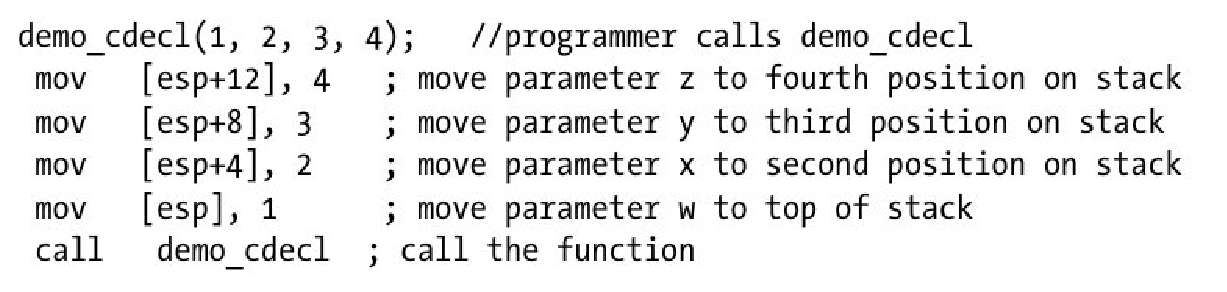
\includegraphics[width=7cm]{images/cdecl_place2.eps}}\\
					\end{column}
				\end{columns}
			\end{figure}
		\end{frame}
		\begin{frame}
			\frametitle{The Standard Calling Convention}
			\begin{itemize}
				\item{This is the Miscrosoft Calling Convention standard}
				\item{When a compiler doesn't use this convention we can force it using the modifier \color{red}\_stdcall}
				\item{Also here the parameters are passed all using only the stack, the difference  is that the called function is responsible for clearing the function parameters from the stack when the function has finished. To do this the function has to know the right number of parameter passed. It's valid only with function with fixed number of parameters so such as printf can't use it.}
				\begin{figure}
					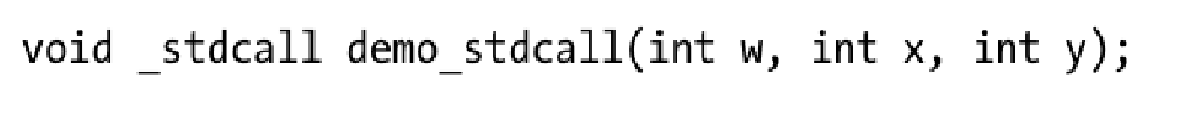
\includegraphics[width=7cm]{images/demo_stdcall.eps}\\
					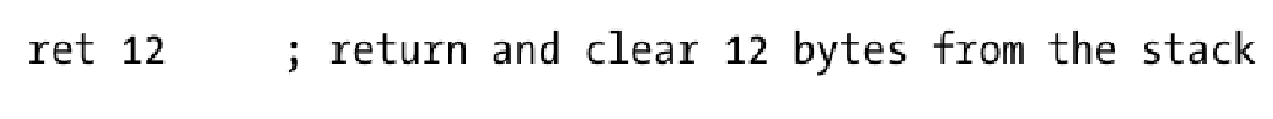
\includegraphics[width=7cm]{images/clear_stack.eps}
				\end{figure}	
			\end{itemize}
		\end{frame}
		\begin{frame}
			\frametitle{fastcall Convention for x86}
			\begin{itemize}
				\item{It's a variation of the stdcall convention, the fastcall  calling convention passes up to two parameters in CPU registers rather than on the program stack.}
				\item{The Microsoft Visual C/ C++ and GNU gcc/g++ compilers recognize the \color{red}fastcall\color{black} modifier in function declaration.}
				\item{In this case the first two parameters are passed in the register (ECX and EDX), the remaining parameters are place on the stack in right to left order similar to stdcall.The function is responsible for removing parameters from the stack when they return to their caller.}
				\begin{figure}
					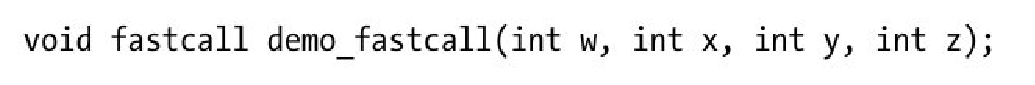
\includegraphics[width=7cm]{images/demo_fastcall.eps}\\
					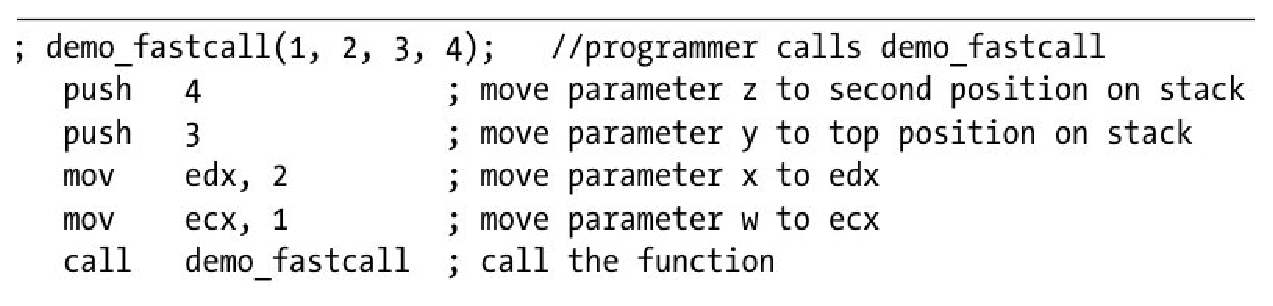
\includegraphics[width=7cm]{images/fastcall_place.eps}\\
				\end{figure}
			\end{itemize}
		\end{frame}

		\begin{frame}
			\frametitle{C++ Calling Convention}
			\begin{itemize}
				\item{This Call Convention is for non static member function in c++ to male available the \textbf{this} pointer-}
				\item{The address of the object used to invoke the function must be supplied by the caller and is therefore provided as a parameter when calling nonstatic member functions.}
				\item{The c++ language standard does not specify how \textbf{this} should be passed to nonstatic member function}
				\item{So here arise the problem that every c++ compiler does something different from another one}
				\item{\color{red} LOOK TO THE SPECIFIC COMPILER WHEN YOU REVERSE C++ PROGRAM!!!}
			\end{itemize}
		\end{frame}
		\begin{frame}
			\frametitle{Other Calling Convention}
			\begin{itemize}
				\item{A Ton of other convention are implemented...They are often language-, compiler- and CPU-specific.}
				\item{Actually all the people that write assembly by hand use the own convention...}
				\item{...Try you to write some little program }
			\end{itemize}
		\end{frame}
\section{Reversing in practice}
	\subsection{Things to know}
		\begin{frame}
		\frametitle{Background of a good Reverser}
			\begin{itemize}
				\item{Assembly Language}
				\item{Compilers}
				\item{Virtual Machine and Bytecodes (ex Java)}
				\item{Operative Systems}
			\end{itemize}
		\end{frame}
	\subsection{Available tools}
		\begin{frame}
			\frametitle{Tools of a good Reverser}
				\begin{itemize}
					\item{System-Monitoring Tools}
					\item{Disassemblers}
					\item{Debuggers}
					\item{Decompilers}
				\end{itemize}
		\end{frame}
		\begin{frame}
			\frametitle{IDA Pro}
				\begin{itemize}
					\item{\textbf{Type:} Disassembler}
					\item{\textbf{Description:} IDApro, without doubts, is the most powerful reverse tool. I will try to resume all the properties of it. It has  three view of the code (graph, text and hex view), a smart version of strings that filter the output to allow a better look at it, two version of the toolbar (advanced and basic), either auto finds data structures inside the code or you can specify it (the same for enums), import/export windows, hexrail extension to get a c-like code of some function, you can specify more than one external debugger to debug your program and much more! }	
				\end{itemize}
		\end{frame}
		\begin{frame}
			\frametitle{OllyDbg}
				\begin{itemize}
					\item{\textbf{Type:} Disassembler and Debugger}
					\item{\textbf{Description:} OllyDbg is a well-known Windows debugger, is really useful on binary code analysis. With OllyDbg is very simple patch the binary to get the desidered flaw of the program. It's really intuitive and you can get it for free online.}
				\end{itemize}
		\end{frame}
		\begin{frame}
			\frametitle{WinDbg}
				\begin{itemize}
					\item{\textbf{Type:} Kernel Debugger}
					\item{\textbf{Description:} This tool is provided by Microsoft, we can use it to debug drivers, applications and services on Windows systems. }
				\end{itemize}
		\end{frame}	
		\begin{frame}
			\frametitle{PEview}
				\begin{itemize}
					\item{\textbf{Type:} Portable Executable(PE) viewer}
					\item{\textbf{Description:} This program is used actually to get a first idea of what is going on. It allows us to see inside the header of the file and understand things such as it's packed or not, it has the resource section with something bad, which are the imports (that's equal to say "What it will try to do in theory on our system")}
				\end{itemize}
		\end{frame}
		\begin{frame}
			\frametitle{Wireshark}
				\begin{itemize}
					\item{\textbf{Type:} Network protocol analyzer}
					\item{\textbf{Description:} WS is a traffic sniffer with a huge set of protocol filter that gives us the full control of what goes on the network. Why do we need it? Actually the reverse engineering process is joint with a dynamic analysis of the malware that maybe uses the network to communicate with remote servers or other bad things. Using wireshark, we can catch and look into every packet that flows in the network. }
				\end{itemize}
		\end{frame}
		\begin{frame}
			\frametitle{Strings}
				\begin{itemize}
					\item{\textbf{Type:} Binary analyzer }
					\item{\textbf{Description:} Strings is a very small program but it can provide us very important information. It looks inside the binary and prints all the printable charaters on the screen. The strings of the binary can be very usuful to understand what is the binary. NB: Ok malware writers are not stupid they will try to put wrong strings inside but if you look at things such as "9.23.111.43" \textbf{maybe} you can suppose that is a ipv4 address and look at it } 
				\end{itemize}			
		\end{frame}
		\begin{frame}
			\frametitle{Snort}
				\begin{itemize}		
					\item{\textbf{Type:} Intrusion detection system}
					\item{\textbf{Description:} It's an open source network intrusion prevention and detection system. We can use it to take under control some event during the execution of a malware. It will give us fast information about new event coming from the network such as a botmaster that send something to our infected test-machine }
				\end{itemize}
		\end{frame}
		\begin{frame}
			\frametitle{Tor}
				\begin{itemize}
					\item{\textbf{Type:} Proxy for Anonymity}
					\item{\textbf{Description:} Tor allows a ton of things, everyone is strictly connected to the \textbf{Anonymity}. The program is a simple proxy that get you access to the "hidden internet". Tor is so anonymous that bad guys, of course, use it to do bad things. Some malware works using tor so we need it to try to undestand its behaviour inside the hidden internet.}
				\end{itemize}
		\end{frame}
		\begin{frame}
			\frametitle{UPX (Ultimate Packer for Executable)}
				\begin{itemize}
					\item{\textbf{Type:} Packer/Unpacker}
					\item{\textbf{Description:} With this program we can detect and unpack malware that use upx packing to avoid antivirus detection. It works on a huge collection of binary format and work on a lot of OS } 
				\end{itemize}
		\end{frame}
		\begin{frame}
			\frametitle{Regshot}
				\begin{itemize}
					\item{\textbf{Type:} Windows register analyzer}
					\item{\textbf{Description:} This tool is designed to make a really simple thing. It allows you to do a snapshot of a the whole set of registers in two different moment and it gives us the differences between snapshot one and two. The result can be used to understand which register are touched by a malware}
				\end{itemize}
		\end{frame}
		\begin{frame}
			\frametitle{Process Monitor}
				\begin{itemize}
					\item{\textbf{Type:} Monitor }
					\item{\textbf{Description:} Process Monitor is an advanced monitoring tool for Windows that shows real-time file system, Registry and process/thread activity. It combines the features of two legacy Sysinternals utilities, Filemon and Regmon, and adds an extensive list of enhancements including rich and non-destructive filtering, comprehensive event properties such session IDs and user names, reliable process information, full thread stacks with integrated symbol support for each operation, simultaneous logging to a file, and much more. Its uniquely powerful features will make Process Monitor a core utility in your system troubleshooting and malware hunting toolkit.}
				\end{itemize}
		\end{frame}
		\begin{frame}
			\frametitle{Process Explorer}
				\begin{itemize}
					\item{\textbf{Type:} Monitor }
					\item{\textbf{Description:} This Program gives us information about either file or directory that are opened by a specific process. The unique capabilities of Process Explorer make it useful for tracking down DLL-version problems or handle leaks, and provide insight into the way Windows and applications work. }
				\end{itemize}
		\end{frame}
		\begin{frame}
			\frametitle{Process Hacker}
				\begin{itemize}
					\item{\textbf{Type:} Monitor}
					\item{\textbf{Description:} Process Hacker is a free and open source process viewer. This multi-purpose tool will assist you with debugging, malware detection and system monitoring. It includes powerful process termination, memory viewing/editing and other unique and specialized features.}
				\end{itemize}
		\end{frame}
		\begin{frame}
			\frametitle{Resource Hacker}
				\begin{itemize}
					\item{\textbf{Type:} Resource section manager}
					\item{\textbf{Description:} Resource HackerTM is a freeware utility to view, modify, rename, add, delete and extract resources in 32bit \& 64bit Windows executables and resource files (*.res). It incorporates an internal resource script compiler and decompiler and works on all (Win95 - Win7) Windows operating systems. }
				\end{itemize}
		\end{frame}
	\subsection{Avoid reversing: how to}
		\begin{frame}
			\frametitle{Reverse on Malware and Antireversing Techniques}
			Today's malware and commercial program use techniques against Reversing
			\begin{itemize}
				\item{Anti-Disassembly (Linear and Flow Oriented Disassembly)}
					\begin{itemize}
						\item{Jump instructions with the same target}
						\item{Jump instruction with a Costant Condition}
						\item{Impossible disassembly}
					\end{itemize}
				\item{Anti-Debugging}
					\begin{itemize}
						\item{They understand that are executed in a debugger and change their behaviour either crashing itself, the debugger or totally doing other stuff}
					\end{itemize}
				\item{Anti-Virtual Machine Techniques}
				\item{Packers and Unpacking}
			\end{itemize}
		\end{frame}
	\subsection{Conclusion}
		\begin{frame}
			\frametitle{Bibliography}
			\begin{itemize}
				\item{The Ida Pro Book 2 Edition }
				\item{The Shellcoder Handbook}
				\item{Reverse Engineering Code with IDA Pro}
				\item{Secrets of Reverse Engineering}
			\end{itemize}
		\end{frame}
	 	\begin{frame}
			\frametitle{Conclusion}
			\begin{itemize}
				\item{Software Reverse Engineering is a very powerfull instrument but it requires a lot of lowlevel-knowledge }
				\item{Appling this technique on malware analysis is not optional if we want undestand how the malware works}
				\item{Can be very time consuming and if all the tools used for the analysis are not setted correctly there's no way to reverse the malware }
			\end{itemize}
		\end{frame}
		\begin{frame}
			\frametitle{End}
			\begin{itemize}
				\item{Thanks Folk...Questions?}
			\end{itemize}
		\end{frame}
%\begin{frame}
%  \frametitle{Simple slide with three points shown in succession}   % Insert frame title between curly braces

%  \begin{itemize}
%  \item<1-> Point 1 (Click ``Next Page'' to see Point 2) % Use Next Page to go to Point 2
%  \item<2-> Point 2  % Use Next Page to go to Point 3
%  \item<3-> Point 3
%  \end{itemize}
%\end{frame}
%\note{Speak clearly}  % Add notes to yourself that will be displayed when
                      % typeset with the notes or notesonly class options



%\begin{frame}
 % \frametitle{Slide with two columns: items and a graphic}   % Insert frame title between curly braces
  %\begin{columns}[c]
 % \column{2in}  % slides are 3in high by 5in wide
 % \begin{itemize}
 %\item<1-> First item
 % \item<2-> Second item
 % \item<3-> ...
 % \end{itemize}
 % \column{2in}
 % \framebox{Insert graphic here % e.g. \includegraphics[height=2.65in]{graphic}
 % }
 % \end{columns}
%\end{frame}
%\note{The end}       % Add notes to yourself that will be displayed when
		     % typeset with the notes or notesonly class options

\end{document}
